\documentclass[10pt,twocolumn,letterpaper]{article}

\usepackage{wacv}
\usepackage{times}
\usepackage{epsfig}
\usepackage{graphicx}
\usepackage{amsmath}
\usepackage{amssymb}
\usepackage{mathtools}
\usepackage{bm}
\usepackage{caption}
\usepackage{subcaption}

% Include other packages here, before hyperref.
\def\ellv{\bm{\ell}}
\def\phiv{{\bm{\phi}}}
\def\thetav{\bm{\theta}}
\def\omegav{\bm{\omega}}

\def\av{\mathbf{a}}
\def\bv{\mathbf{b}}
\def\cv{\mathbf{c}}
\def\dv{\mathbf{d}}
\def\ev{\mathbf{e}}
\def\fv{\mathbf{f}}
\def\gv{\mathbf{g}}
\def\hv{\mathbf{h}}
\def\iv{\mathbf{i}}
\def\jv{\mathbf{j}}
\def\kv{\mathbf{k}}
\def\lv{\mathbf{l}}
\def\mv{\mathbf{m}}
\def\nv{\mathbf{n}}
\def\ov{\mathbf{o}}
\def\pv{\mathbf{p}}
\def\qv{\mathbf{q}}
\def\rv{\mathbf{r}}
\def\sv{\mathbf{s}}
\def\tv{\mathbf{t}}
\def\uv{\mathbf{u}}
\def\vv{\mathbf{v}}
\def\wv{\mathbf{w}}
\def\xv{\mathbf{x}}
\def\yv{\mathbf{y}}
\def\zv{\mathbf{z}}

\def\Am{\mathbf{A}}
\def\Bm{\mathbf{B}}
\def\Cm{\mathbf{C}}
\def\Dm{\mathbf{D}}
\def\Em{\mathbf{E}}
\def\Fm{\mathbf{F}}
\def\Gm{\mathbf{G}}
\def\Hm{\mathbf{H}}
\def\Im{\mathbf{I}}
\def\Jm{\mathbf{J}}
\def\Km{\mathbf{K}}
\def\Lm{\mathbf{L}}
\def\Mm{\mathbf{M}}
\def\Nm{\mathbf{N}}
\def\Om{\mathbf{O}}
\def\Pm{\mathbf{P}}
\def\Qm{\mathbf{Q}}
\def\Rm{\mathbf{R}}
\def\Sm{\mathbf{S}}
\def\Tm{\mathbf{T}}
\def\Um{\mathbf{U}}
\def\Vm{\mathbf{V}}
\def\Wm{\mathbf{W}}
\def\Xm{\mathbf{X}}
\def\Ym{\mathbf{Y}}
\def\Zm{\mathbf{Z}}

\newcommand{\homogeneous}[1]{\hat{#1}} % Vector homogenous notation
\newcommand{\hnorm}[1]{\check{#1}} % Perspective division notation

\def\Projection{\mathcal{P}}
\def\IntrinsicMatFunc{\mathcal{K}}
\def\ExtrinsicFunc{\mathcal{R}}
\def\pdiv{\hat{\mathbf{\nu}}}
\def\Distortion{\mathcal{D}}

\def\Real{\varmathbb{R}}
\def\Projective{\varmathbb{P}}

\DeclareMathOperator*{\argmin}{arg\,min}
\DeclareMathOperator{\Err}{Err}
\DeclareMathOperator{\Proj}{Proj}
\DeclareMathOperator{\Norm}{Norm}

\DeclarePairedDelimiter{\norm}{\lVert}{\rVert}

% Add a period to the end of an abbreviation unless there's one
% already, then \xspace.
\makeatletter
\DeclareRobustCommand\onedot{\futurelet\@let@token\@onedot}
\def\@onedot{\ifx\@let@token.\else.\null\fi\xspace}

\def\eg{\emph{e.g}\onedot} \def\Eg{\emph{E.g}\onedot}
\def\ie{\emph{i.e}\onedot} \def\Ie{\emph{I.e}\onedot}
\def\cf{\emph{c.f}\onedot} \def\Cf{\emph{C.f}\onedot}
\def\etc{\emph{etc}\onedot} \def\vs{\emph{vs}\onedot}
\def\wrt{w.r.t\onedot} \def\dof{d.o.f\onedot}
\def\etal{\emph{et al}\onedot}
\makeatother

%Author notes
\def\authornote#1#2{{\textred{\textsl{\small#1:[*#2*]}}}} \newcommand*{\Scale}[2][4]{\scalebox{#1}{$#2$}}%
\newcommand{\dhnote}[1]{\authornote{DH}{#1}} % Daniel
\newcommand{\jknote}[1]{\authornote{JK}{#1}} % Juho
\newcommand{\jhnote}[1]{\authornote{JH}{#1}} % Janne

\graphicspath{{images/}}

% If you comment hyperref and then uncomment it, you should delete
% egpaper.aux before re-running latex.  (Or just hit 'q' on the first latex
% run, let it finish, and you should be clear).
\usepackage[pagebackref=true,breaklinks=true,letterpaper=true,colorlinks,bookmarks=false]{hyperref}

\wacvfinalcopy % *** Uncomment this line for the final submission

\def\wacvPaperID{287} % *** Enter the CVPR Paper ID here
\def\httilde{\mbox{\tt\raisebox{-.5ex}{\symbol{126}}}}

% Pages are numbered in submission mode, and unnumbered in camera-ready
\ifwacvfinal\pagestyle{empty}\fi
\begin{document}

%%%%%%%%% TITLE
\title{Forget the checkerboard: practical self-calibration using a planar scene}

\author{Daniel Herrera C. \qquad Juho Kannala \qquad Janne Heikkil\"a\\
University of Oulu\\
Finland\\
%{\tt\small daniel.herrera.castro@gmail.com}
% For a paper whose authors are all at the same institution,
% omit the following lines up until the closing ``}''.
% Additional authors and addresses can be added with ``\and'',
% just like the second author.
% To save space, use either the email address or home page, not both
%\and
%Second Author\\
%Institution2\\
%First line of institution2 address\\
%{\tt\small secondauthor@i2.org}
%\and Juho Kannala \and Janne Heikkil\"a
}

\maketitle
%\thispagestyle{empty}


%%%%%%%%% ABSTRACT
\begin{abstract}
We introduce a camera self-calibration method using a planar scene of unknown texture. Planar surfaces are everywhere but checkerboards are not, thus the method can be more easily applied outside the lab. We demonstrate that the accuracy is equivalent to a checkerboard-based calibration, so there is no need for printing checkerboards any more. Moreover, the use of a planar scene provides improved robustness and stronger constraints than a self-calibration with an arbitrary scene. We utilize a closed-form initialization of the focal length with minimal and practical assumptions. The method recovers the intrinsic and extrinsic parameters of the camera and the metric structure of the planar scene. The method is implemented in a real-time application for non-expert users that provides an easy and practical process to obtain high accuracy calibrations. 
\end{abstract}

%%%%%%%%% BODY TEXT	
\section{Introduction}

Calibrating a camera's intrinsics (focal length, principal point, and distortion coefficients) is a fundamental problem in computer vision. A calibrated camera is needed to perform a metric reconstruction of a scene, otherwise only a projective reconstruction is possible \cite{hartley2003}. Some of the most interesting applications of computer vision, like simultaneous localization and mapping, augmented reality, and 3D reconstruction, require a metric reconstruction of the scene. Nowadays, cameras are most often calibrated offline using a calibration target. A planar target with a checkerboard or circular pattern of known structure is a well established and popular method for camera calibration \cite{sturm1999,zhang1999,bouguetMCT,kannala2008}.

%Why is homography-based calibration important? Practical (easy targets) and accurate (homographies are robust to point noise)
Planar scenes are a very convenient calibration target because they are easy to detect, match, and the observed motion can be completely described by a homography. A planar target is much easier to manufacture than a 3D target of known structure, for example a paper checkerboard can be produced by a standard printer and attached to a table. Homography-based known-target calibration methods like \cite{sturm1999,zhang1999} extract the intrinsic parameters of a camera from a set of homographies between the known points in metric space and the matched points in image space. This produces a very accurate calibration because the homographies are very robust to noise and outliers. 

%Why is homography-based self-calibration important? Even more practical (targets everywhere) and still accurate (strong planar constraint)
Although this is an accurate and practical method, it is not as practical as it can be. Checkerboard targets are often inconvenient and not always available, especially outside the lab. There are a myriad of well-textured planar targets in the wild (books, paintings, billboards) but the metric structure of their texture is not known a-priori and are thus not suited for a method like \cite{zhang1999}. We explore the problem of \emph{planar self-calibration} which attempts to simultaneously calibrate the camera and recover the metric structure of the scene under the assumption that the scene is planar. 

Planar self-calibration is attractive for several reasons. It is much more practical than a known-target calibration because we can use any planar structure for calibration. On the other hand, when compared to a generic self-calibration approach, the planar-scene constraint significantly reduces the degrees of freedom of the problem and increases the robustness and accuracy of the calibration. Moreover, homography estimation is a much simpler and robust process than feature matching of arbitrary 3D points.

%Why is it hard? Generic self-calibration has linear solution, but planar doesn't.
An internal and necessary component of planar self-calibration is \emph{homography-based self-calibration} which takes a set of homographies and estimates the intrinsic parameters of the camera. So far, homography-based self-calibration has been proven possible \cite{triggs1998} but it has not led to a practical implementation that can replace known-target calibration methods due to its lack of a closed-form solution for initialization. Checkerboard-based calibration is still the standard calibration technique due to several reasons. Homography-based self-calibration by itself cannot reach the accuracy of a known-target calibration because the camera poses are implicitly fixed within the homographies. There hasn't been a proper comparison of the performance of both calibration types that would prove that it is safe to use planar self-calibration without sacrificing accuracy. Moreover, there is no publicly available implementation as there is for known-target calibration, \eg \cite{bouguetMCT}. 

In this paper we address these issues and describe a complete planar self-calibration system that rivals the performance of known-target calibration methods. We compare the limits of both calibration types and show that in almost any practical situation, planar self-calibration can be used to obtain calibrations with the same accuracy as that of known-target calibration methods.

%not been a viable option because the non-linearities introduced by the planar-scene constraint have prevented a closed-form solution. A closed-form solution for the camera intrinsics, and for the focal length in particular, is fundamental to initialize a non-linear optimization of the self-calibration constraints which is easily trapped in local minima. In this paper we show that a closed-form solution for the focal length is possible by imposing a minor constraint on the camera motion: the scene plane should be close to fronto-parallel to at least one image in the dataset. We believe this limitation is insignificant in practice and results in a system that can be easily and robustly used in the wild to perform accurate calibration.

\subsection*{Previous work}

Hartley and Zisserman \cite{hartley2003} present a comprehensive analysis of camera calibration, including known-target and self-calibration methods. In the area of known-target calibration the landmark paper of Zhang \cite{zhang1999} is nowadays the defacto standard for camera calibration and has been implemented for many platforms \cite{bouguetMCT,opencv_library}. It is interesting to notice that the calibration constraints used there have the same nature as the ones presented here. However, because the metric structure of the world is known the equations simplify considerably, there are less degrees of freedom, and the optimization is performed directly in metric space. 

There has been considerable progress in the area of self-calibration when the observed scene has a 3D structure. Closed-form and linear solutions have been obtained to recover the focal length of a moving camera \cite{bougnoux1998}. However, these methods fail when the scene is planar. The planar self-calibration constraints were first introduced by Triggs \cite{triggs1998}. Triggs encoded the plane structure with two circular points using 4 degrees of freedom (DoF). Bocquillon \etal \cite{bocquillon2006} later reformulated these constraints to encode the plane structure using only the plane normal (2 DoF) and solved the calibration problem using interval analysis which results in an exhaustive search through parameter space.

Gurdjos and Sturm \cite{gurdjos2003} took a different approach using the \emph{centre line constraint}. Their formulation keeps the DoF constant even with a varying focal length. However, it is less constrained than the formulation of \cite{bocquillon2006} and requires more images to reach the same accuracy. Gurdjos and Sturm also provide a closed-form solution under a minor assumption, namely that the reference image is close to fronto-parallel with the scene plane.

Our system combines the ideas from \cite{bocquillon2006} and \cite{gurdjos2003} and extends them into a complete planar self-calibration system. We take a novel approach to derive the homography-based self-calibration constraints which highlights a weakness of the existing formulation. We solve this by providing a new set of normalized constraints. We use the same assumption as \cite{gurdjos2003} to obtain a closed-form solution and bootstrap the calibration. Then, we obtain a significant improvement in the final accuracy by normalizing the constraints and adding a final bundle adjustment in metric space. Our contributions can be summarized as follows
\begin{itemize}

\item A new set of normalized planar self-calibration constraints that are more robust to noise.

\item A novel derivation of the planar self-calibration constraints that is more intuitive and provides insight into the nature of the constraints.

\item A complete planar self-calibration pipeline that robustly obtains a final metric reconstruction and calibration with an accuracy significantly higher than that of a homography-based self calibration.

\item A direct comparison of the accuracy of planar known-target and self-calibration methods.

\item An open source implementation of the planar self-calibration system.

\end{itemize}

\begin{figure}
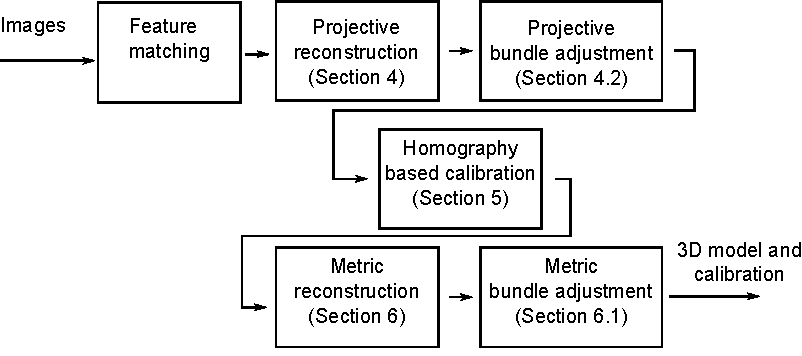
\includegraphics[width=\linewidth]{images/pipeline.pdf}
\caption{The outline of our planar self-calibration algorithm. It first performs a projective reconstruction, then recovers the calibration matrix from the obtained homographies, and then upgrades it to a metric reconstruction.}
\label{fig:diagram}
\end{figure}

\section{The planar self-calibration system}

The homography-based self-calibration stage as described by \cite{bocquillon2006} and \cite{gurdjos2003} is a key component for planar self-calibration but it is not enough to produce the best calibration results. A projective reconstruction stage is needed before it to prepare the homographies and a metric recronstruction stage is needed after it to perform a final bundle adjustment. The structure of the final system is shown in Fig.~\ref{fig:diagram}. We first describe our camera model in Section \ref{sec:camera}.

The projective reconstruction stage receives the input images and extracts the homographies between them. It also gives an initial estimate of the distortion. It initially estimates each homography individually and then performs a global bundle adjustment of all homographies, the distortion coefficients, and the observed points in projective space. Section \ref{sec:projective} describes this stage in detail.

Once the optimal set of homographies is found, they are fed into a homography-based self-calibration stage that simultaneously recovers the camera calibration and the pose of the reference camera. We derive the planar self-calibration constraints and propose a novel set of normalized constraints in Section \ref{sec:calib}.

The calibration obtained allows a metric reconstruction of the scene. However, this calibration is not optimal because the camera poses were not optimized together with the intrinsic parameters. Thus, a metric reconstruction is performed and a final bundle adjustment is done to obtain the optimal calibration. Details of this reconstruction and final optimization are described in Section \ref{section:metric}.

%The following sections describe each stage in detail. The feature matching stage is not described since it can be implemented with any standard feature descriptor and matching approach, \eg \cite{rublee2011orb}.

~\\ \noindent\textbf{Notation:}
We denote vector quantities as bold lowercase letters (\eg $\xv$,$\pv$,$\tv$), matrix quantities as bold uppercase letters (\eg $\Rm$,$\Km$), and scalars as lowercase italic letters (\eg $f_x$,$u_0$). We denote the homogeneous representation of a vector $\xv$ with $\homogeneous{\xv}$. The transformation back from homogeneous coordinates, denoted by $\hnorm(\homogeneous{\xv})$, is performed by dividing a vector by its last component and discarding it. 
%Equations in homogeneous coordinates are equal up to scale and this is denoted by the $\propto$ symbol.
%We frequently change between homogeneous and inhomogeneous representation of vectors.


\section{Camera model}
\label{sec:camera}

We model our camera using the well-known pinhole model with radial distortion. The projection function $\pv=\Projection(\xv)$ transforms a point in 3D world space $\xv=[x,y,z]^\top$ to a 2D pixel position $\pv=[u,v]^\top$. The projection function is the composition of three functions: the extrinsic transform $\ExtrinsicFunc$, the intrinsic transform $\IntrinsicFunc$, and the distortion function $\Distortion$, \ie $\Projection(\xv) = \Distortion \circ \IntrinsicFunc \circ \ExtrinsicFunc(\xv)$.

The extrinsic transform is a rigid 3D transform that aligns the point with the camera reference frame
%
\begin{align}
\xv_c &= \ExtrinsicFunc(\xv) = \Rm \xv + \tv 
\end{align}
%
where the rotation matrix $\Rm$ and the translation vector $\tv$ are the extrinsic parameters of the camera, \ie its rigid pose. The intrinsic function converts the point from metric to pixel units
%
\begin{align}
\pv_n &= \IntrinsicFunc(\xv_c) = \hnorm(\Km \xv_c)
\\
\Km &= \begin{bmatrix}
f_x & 0 & u_0 \\
0 & f_y & v_0 \\
0 & 0 & 1
\end{bmatrix}
\label{eq:intrinsic_matrix}
\end{align}.
%

Finally, the distorted point is obtained by applying
%
\begin{align}
\pv = \Distortion(\pv_n) &= (\pv_n-\pv_0) (1+r^2 d_0 + r^4 d_1) + \pv_0
\label{eq:distortion}
\end{align}
%
where $\pv_0=[u_0,v_0]^\top$ is the principal point and $r = \norm{\pv_n - \pv_0}$. The vector $\dv=[d_0,d_1]^\top$ contains the distortion coefficients. 

The camera model contains 6 degrees of freedom (DoF) for the extrinsic parameters (three for rotation and three for translation) and 6 DoF for the intrinsic parameters (two focal lengths, two for the principal point, and two distortion coefficients). 

%%%%%%%%%%%%%%%%%%%%%%%%%%%%%%%%%%%%%%%%%%%%%%%%%%%%%%%%%%%%%%%%%%%%
%% Projective
%%%%%%%%%%%%%%%%%%%%%%%%%%%%%%%%%%%%%%%%%%%%%%%%%%%%%%%%%%%%%%%%%%%%
\section{Projective reconstruction}
\label{sec:projective}

Planar geometry is well understood and extensively documented. Here we provide a brief review of what is relevant to this paper. Further details can be found in \cite{hartley2003}. We first approach planar geometry using a pinhole camera with no distortion. Section \ref{sec:planar:distortion} addresses the effects of distortion.

A planar scene induces a homography between two pinhole cameras. That is, the measurements of image $i$ are related to those of image $j$ by
%
\begin{align}
\homogeneous{\pv}_j \propto \Hm_{ij} \homogeneous{\pv}_i 
\label{eq:homography}
\end{align}
%
where $\Hm_{ij}$ is a $3 \times 3$ full-rank matrix. The equation is only up to scale because all elements are in homogeneous coordinates and thus $\Hm_{ij}$ has only 8 DoF.

The first step in our algorithm is to obtain a projective reconstruction of the scene. The reconstruction includes the position of the observed points in world coordinates and the poses of the cameras. The points can be represented with a 2D position vector $\yv=[x,y]^\top$ because the scene is planar. The pose of a camera $i$ can be represented by a homography $\Hm_i$ that translates the points from world to image space. 

A projective reconstruction is defined up to a homography. Thus, without loss of generality we select one of the image frames as the reference frame, say image $0$, which has the same coordinate frame as the world, \ie $\Hm_0 = \Im_{3 \times 3}$. This also implicitly fixes the position of the world points $\yv=\pv_0$. The poses of the other frames can be determined independently by computing the homography between them and the reference frame.

\subsection{Distortion}
\label{sec:planar:distortion}

The relation of Eq.~\eqref{eq:homography} only holds for a pinhole camera without distortion. In the case of distortion, the undistorted measurements will still follow Eq.~\eqref{eq:homography}. We can thus estimate the distortion model by finding the coefficients that allow the measurements to be modelled by a homography. We use the distortion model from Eq.~\eqref{eq:distortion} to remove the distortion in image space.

Although there are methods of estimating the distortion parameters from a set of uncalibrated images, for simplicity we rely here on robust homography estimation methods \cite{hartley2003} to obtain an initial projective reconstruction assuming no distortion. The distortion coefficients are then estimated during a projective bundle adjustment step. This has proven to work well with moderate distortion levels.

\subsection{Projective bundle adjustment}
\label{sec:projective:ba}

The projective reconstruction obtained so far is not optimal for two reasons. First, the homographies have all been computed in a pair-wise manner between the reference image and the all others. This ignores the fact that the other images might constrain each other's projective pose as well. In fact, as the camera moves farther away from the reference pose, matching becomes harder and nearby images might constrain the pose better. Second, distortion has not been estimated yet. Even under mild distortion, this can add a considerable noise to homographies that are estimated from distorted pixel correspondences.

Although the final metric bundle adjustment might recover from these intermediate errors, there is no guarantee. Thus, we perform a robust non-linear minimization \cite{ceres-solver} over all parameters to obtain the optimal projective reconstruction. The formulation of the minimization problem is as follows, 
%
\begin{align}
\argmin_{\dv',\pv_0,\lbrace \Hm_i \rbrace, \lbrace \yv_k \rbrace} 
%
\sum_i \sum_k \rho(\norm{\pv_{ik} - \Distortion(\Hm_i \yv_k)})^2 + \lambda\norm{\pv_0 - \bar{\pv}_0}^2
\end{align}
%
where $\rho(\cdot)$ is a robust function to reduce the influence of outliers (\eg the Cauchy loss function \cite{ceres-solver}). The first term transforms the projective positions of a point $\yv_k$ to the frame of camera $i$ through its homography $\Hm_i$, distorts it, and compares it with the measured position $\pv_{ik}$. The homography of the reference camera is kept fixed to remove the projective ambiguity. However, all point coordinates $\yv_j$ are optimized to remove any bias towards the reference camera. The final term regularizes the center of distortion, biasing it towards the center of the image $\bar{\pv}_0$ in case of no distortion. The weighting term $\lambda$ is set to the inverse of the expected variance of the principal point. However, this regularization is only a safety measure and is negligible with even minor distortions.

%%%%%%%%%%%%%%%%%%%%%%%%%%%%%%%%%%%%%%%%%%%%%%%%%%%%%%%%%%%%%%%%%%%%
%% Calibration
%%%%%%%%%%%%%%%%%%%%%%%%%%%%%%%%%%%%%%%%%%%%%%%%%%%%%%%%%%%%%%%%%%%%
\section{Homography-based self-calibration}
\label{sec:calib}

We first derive the constraints for homography-based self-calibration. We take a different route than \cite{bocquillon2006} for clarity and to gain insight into the nature of the constraints. Yet, the constraints obtained in this section are equivalent to those of \cite{bocquillon2006}, as is shown in Section \ref{sec:calib:connection}. In Section \ref{sec:calib:normalization} we show that these constraints are biased and propose a new set of normalized constraints. We then derive a closed-form solution to obtain an initial guess for the focal length in Section \ref{sec:calib:closed}.

The input to a homography-based self-calibration stage are a series of homographies $\lbrace \Hm_i \rbrace$ that relate all images to a reference image. The calibration recovers the intrinsic parameters $f_x$,$f_y$, and $\pv_0$. It assumes no distortion since the distortion has been corrected beforehand during the projective reconstruction stage.

The calibration constraints come from our knowledge of the metric structure of the world applied to the obtained projective reconstruction. To derive the constraints we arbitrarily choose our metric world coordinate frame to coincide with the camera frame of the reference image. We describe the scene plane in this reference frame by its 3D normal vector $\nv_0$ (with unit norm) and the distance to the origin.

We encode the Euclidean structure of the plane with two orthogonal basis vectors with equal norm that span the plane: $\av_0$ and $\bv_0$. Like the normal vector, these vectors represent directions in 3D space, see Fig.~\ref{fig:planar_structure}. Note that these vectors are not unique since we can rotate them around $\nv_0$ and they are still orthonormal basis vectors. With this in mind, the following equations encode the orthogonality and equal norm constraints respectively
\begin{align}
\av_i^\top \bv_i = 0, \label{eq:ortho_constraint} \\
\av_i^\top \av_i - \bv_i^\top \bv_i = 0, \label{eq:norm_constraint}
\end{align}
where the index $i$ has been kept variable because these constraints apply to all cameras.

\begin{figure}
\centering
\input{images/basisVectors.pdf_tex}
\caption{Planar self-calibration geometry.}
\label{fig:planar_structure}
\end{figure}

By definition, we can derive these vectors for the reference camera. To ensure orthogonality, we select $\av_0$ as the cross product of $\nv_0$ with an auxiliary fixed vector $\ev$
\begin{align}
\av_0 = \nv_0 \times \ev = [\nv_0]_\times \ev \\
\bv_0 = \nv_0 \times \av_0 = [\nv_0]_\times^2 \ev
\end{align}
Note that $\ev$ can be any vector as long as it is not parallel to $\nv_0$. A different $\ev$ will produce a different orientation for the basis but Eqs.~\eqref{eq:ortho_constraint} and \eqref{eq:norm_constraint} will remain unchanged.

Given the basis vectors in the reference camera they can be transformed to the frame of camera $i$ through its homography
\begin{align}
\av_i = \Km^{-1} \Hm_i \Km \av_0, \\
\bv_i = \Km^{-1} \Hm_i \Km \bv_0.
\end{align}
%
Note that Eqs.~\eqref{eq:ortho_constraint} and \eqref{eq:norm_constraint} for the reference camera are satisfied by definition but the other cameras constrain $\Km$ using the reconstructed homographies. These are the self-calibration constraints that will allow us to recover $\Km$.

\subsection{Connection with previous work}
\label{sec:calib:connection}

Although our derivation takes a different route, the constraints obtained so far are identical to those proposed in \cite{bocquillon2006}. The components of the \emph{circular points} in \cite{bocquillon2006} $\xv_1$ and $\xv_2$ are simply the images of the basis vectors (\ie $\xv_1=\Km \av_0$ and $\xv_2=\Km \bv_0$). By using the notation $\omega=\Km^{-\top}\Km^{-1}$, Eqs.~\eqref{eq:ortho_constraint} and \eqref{eq:norm_constraint} can be expanded to be expressed as in \cite{bocquillon2006}
%
\begin{align}
\av_i^\top \bv_i &= (\Km^{-1} \Hm_i \Km \av_0)^\top (\Km^{-1} \Hm_i \Km \bv_0) \notag \\
%&= (\Km^{-1} \Hm_i \xv_1)^\top (\Km^{-1} \Hm_i \xv_2) \notag \\
&= \xv_1^\top \Hm_i^\top \omegav \Hm_i \xv_2 = 0 
\\
\av_i^\top \av_i - \bv_i^\top \bv_i &= (\Km^{-1} \Hm_i \Km \av_0)^\top (\Km^{-1} \Hm_i \Km \av_0) \notag 
\\
&\quad - (\Km^{-1} \Hm_i \Km \bv_0)^\top (\Km^{-1} \Hm_i \Km \bv_0) \notag 
\\
%&= (\Km^{-1} \Hm_i \xv_1)^\top (\Km^{-1} \Hm_i \xv_1) \notag 
%\\
%&\quad - (\Km^{-1} \Hm_i \xv_2)^\top (\Km^{-1} \Hm_i \xv_1) \notag 
%\\
&= \xv_1^\top \Hm_i^\top \omegav \Hm_i \xv_1 - \xv_2^\top \Hm_i^\top \omegav \Hm_i \xv_2 = 0 
\end{align}
which are the same constraints and with the same parametrization as in Eq.~(4) of \cite{bocquillon2006}. The resulting unknowns are $\Km$ and $\nv_0$. The normal $\nv_0$ has 3 variables with 2 DoF. The intrinsic matrix $\Km$ varies between 5 DoF and 1 DoF depending on the camera model. Vector $\ev$ is not an unknown of the problem. It can be chosen arbitrarily and fixed as long as it is not parallel to the normal vector.


\subsection{Closed-form with a known plane normal}
\label{sec:calib:closed}

The normalized constraints can be readily used in an iterative non-linear minimization procedure to find the optimum values for the intrinsic parameters and the normal vector. However, we need an initial guess that we'd like to obtain in closed-form. A closed-form solution can be obtained if we assume a known plane normal and a simplified camera model. Gurdjos and Sturm \cite{gurdjos2003} derived a closed-form solution using their formulation. Here we show that our formulation so far is equivalent and reaches the same closed-form solution.

%We reduce the intrinsic matrix to have 1 DoF by assuming a single focal length and a known principal point. We use the distortion center obtained from a projective reconstruction as the principal point and translate the obtained homographies so that this point lies in the origin. The intrinsic matrix is then $\Km=\text{diag}(f, f, 1)$. 

We reduce the intrinsic matrix to have 1 DoF, \ie $\Km=\text{diag}(f, f, 1)$, and assume a reference image fronto-parallel to the plane, \ie $\nv_0=[0,0,1]^\top$. This seems like a strong assumption, however it is only used to obtain an initial guess of the focal length. The constraint is dropped during the optimization step and the real normal is found. Moreover, different initial guesses for the focal length can be obtained very cheaply by repeating this procedure with a different input image selected as the reference frame. The best initial guess from these can then be used for further optimization. The experiments presented in Section \ref{sec:results} demonstrate the robustness of the algorithm to violations of this assumption.

Under these assumptions the constraints \eqref{eq:ortho_constraint} and \eqref{eq:norm_constraint} reduce to a pair of quadratic polynomials in one variable 
\begin{align}
h_{31}\, h_{32}\, f^2 + h_{11}\, h_{12} + h_{21}\, h_{22}=0
\label{eq:closed_form_a}
\\
f^2\, {h_{31}}^2 - f^2\, {h_{32}}^2 + {h_{11}}^2 + {h_{21}}^2 - {h_{12}}^2 - {h_{22}}^2=0
\label{eq:closed_form_b}
\end{align}
Note that since $\nv_0$ is known the choice of $\ev$ vanishes. Choosing either $\ev=[1,0,0]^\top$ or $\ev=[0,1,0]^\top$ result in the same equations. However, choosing $\ev=[0,0,1]^\top$ (\ie $\ev=\nv_0$) results in the trivial constraint $0=0$. Each homography imposes two constraints on the focal length. Since the focal length only appears in quadratic form Eqs.~\eqref{eq:closed_form_a} and \eqref{eq:closed_form_b} simplify to linear constraints that can the be solved directly as an overdetermined linear system to obtain $f$. In case of outliers, a RANSAC approach can be used here to discard homographies that were poorly estimated.

\subsection{Scale and normalization}
\label{sec:calib:normalization}

In the absence of noise, the self-calibration constraints are homogeneous and their scale does not matter. However, with real data the constraints will have non-zero residuals and their scale affects the solution obtained. For example, Eq.~\eqref{eq:ortho_constraint} can also be expressed as
\begin{align}
\av_i^\top \bv_i = \norm{\av_i} \norm{\bv_i} \cos \theta_{a_i b_i}
\end{align} 
where $\theta_{a_i b_i}$ is the angle between the vectors. We see that the scale of the residuals is directly proportional to the norm of the vectors. However, this constraint should only depend on the angle because it is an orthogonality constraint. Similarly, Eq.~\eqref{eq:norm_constraint} should only constrain the norms of the vectors to be equal regardless of their scale. The constraints from both \cite{bocquillon2006} and \cite{gurdjos2003} suffer from this problem.

%
There are two factors that affect the norm of the basis vectors: the homography's scale and the angle between $\nv_0$ and $\ev$, \ie
%
\begin{align}
\norm{\av_i} \propto \norm{\Hm_i} \sin \theta_{\nv_0 \ev}
\end{align} 
%
Both of these bias the calibration process if not accounted for. A homography is a homogenous quantity and can have any arbitrary scale. For example, if it is obtained through linear means, it is usual to set $h_{33}=1$ and thus fix the scale. However, if it is obtained through SVD it is common to set $||\Hm||_F=1$. Even though they are equivalent, these two normalizations produce very different results when using constraints \eqref{eq:ortho_constraint} and \eqref{eq:norm_constraint}, because they give a different and unequal weight to the residuals. 

In a similar fashion, the angle between $\nv_0$ and $\ev$ will also bias the solution. Even though $\ev$ can be fixed, the normal of the plane will vary during the optimization. A larger angle will lead to a smaller norm for the basis vectors, thus reducing the cost of the solution and biasing the optimization towards larger angles between $\nv_0$ and $\ev$. In the extreme, when the vectors are perpendicular, all residuals vanish. 
%
Even if $\ev$ is adjusted after each iteration to avoid vanishing residuals, it is not possible to normalize the homographies to give an equal norm to all basis vectors. To remove this bias and improve the obtained calibration we propose a pair of normalized constraints that are scale independent
%
\begin{align}
\cos \theta_{a_i b_i} = \frac{\av_i \cdot \bv_i}{\norm{\av_i} \norm{\bv_i}} &= 0 \label{eq:ortho_constraint_normalized}\\
1 - \frac{\norm{\bv_i}^2}{\norm{\av_i}^2} &= 0 \label{eq:norm_constraint_normalized}
\end{align}
These constraints are shown in Section \ref{sec:results} to produce a more stable and accurate calibration than the original constraints of \cite{bocquillon2006} and \cite{gurdjos2003}. 

Normalizing the homographies with their Frobenious norm is recommended to avoid possible singularities \cite{hartley2003}. We still tried both normalizations for the homographies and our normalized constraints consistently produced a better calibration in both cases. 

%\subsection{Minimal configuration}
%
%According to \cite{hartley2003} the problem of planar calibration is well constrained when $2m \geq v+4$ where $m$ is the number of views and $v$ is the DoF of the intrinsic parameters. However, \cite{hartley2003} used 4 DoF for the circular points. The current formulation makes these a function of the normal vector and thus reduces them to 2 DoF. Thus, the minimal configuration requires $2m \geq v+2$. For example, if we only want to estimate the focal length ($2m \geq 1+2$) one homography is enough, as demonstrated by Eqs.~\eqref{eq:closed_form_a} and \eqref{eq:closed_form_b}.

\subsection{Non-linear optimization}

The closed-form solution provides an initial guess under the fixed-normal assumption. Although rough, this is a suitable starting point for a non-linear optimization using the constraints \eqref{eq:ortho_constraint_normalized} and \eqref{eq:norm_constraint_normalized}. The formulation of the minimization problem is as follows, 
%
\begin{align}
\argmin_{\Km,\nv_0} 
\sum_i 
\frac{\av_i \cdot \bv_i}{\norm{\av_i} \norm{\bv_i}} +
\sum_i 
1 - \frac{\norm{\bv_i}^2}{\norm{\av_i}^2}
\label{eq:calib_ba}
\end{align}
%
where the normal vector is constrained to have unit norm and $\Km$ is allowed to have 4 DoF as in \eqref{eq:intrinsic_matrix}. Although this non-linear minimization is necessary to improve the initial guess, it is still not optimal because the camera poses are encoded into the homographies and cannot be optimized. The optimal solution will be obtained by optimizing in metric space.

%%%%%%%%%%%%%%%%%%%%%%%%%%%%%%%%%%%%%%%%%%%%%%%%%%%%%%%%%%%%%%%%%%%%
%% Metric
%%%%%%%%%%%%%%%%%%%%%%%%%%%%%%%%%%%%%%%%%%%%%%%%%%%%%%%%%%%%%%%%%%%%
\section{Metric reconstruction}
\label{section:metric}

Once the intrinsic parameters have been recovered, upgrading the projective reconstruction to a metric reconstruction is straightforward. We define a new world reference frame so that the scene's plane lies at $z=0$. Under this reference frame, the extrinsic parameters of the reference camera are initialized to $\Rm=[\av, \bv, \nv]^\top$ and $\tv= - \Rm \nv$, which positions the camera exactly one unit away from the plane center and aligns it with the recovered normal.

The position $\xv=[x,y,0]$ of the observed points can be obtained by intersecting the optical ray of the reference camera with the scene plane at $z=0$. The extrinsic parameters of the other cameras are implicitly contained in the homographies and could be directly recovered from them using non-linear means. Alternatively, since the observed points are already triangulated and the camera is calibrated we can use well-known perspective-n-points techniques to estimate the extrinsics \cite{quan1999}.

This produces a complete and calibrated 3D reconstruction of the scene and the cameras, including the intrinsic parameters, $\Km$ and $\dv$, the extrinsic parameters, $\lbrace \Rm_i \rbrace$ and $\lbrace \tv_i \rbrace$, and the point 3D positions, $\lbrace \xv_k \rbrace$.

\subsection{Metric bundle adjustment}

The final solution is obtained by a non-linear optimization which minimizes the reprojection errors of 3D points on image space. That is, the point coordinates are now in metric space and the quantity minimized is in pixel units. This implicitly enforces all known constraints about the scene over all measurements. The formulation of the minimization problem is as follows, 
%
\begin{align}
\argmin_{\Km,\dv,\lbrace \Rm_i \rbrace,\lbrace \tv_i \rbrace, \lbrace \xv_k \rbrace} 
%
\sum_i \sum_k \rho(\norm{\pv_{ik} - \Projection_i(\xv_k))})^2 
\end{align}
%
where the position of the points is constrained so that $z=0$. 

%%%%%%%%%%%%%%%%%%%%%%%%%%%%%%%%%%%%%%%%%%%%%%%%%%%%%%%%%%%%%%%%%%%%
%% Results
%%%%%%%%%%%%%%%%%%%%%%%%%%%%%%%%%%%%%%%%%%%%%%%%%%%%%%%%%%%%%%%%%%%%
\section{Experimental results}
\label{sec:results}

We present a series of experiments that highlight the accuracy, robustness, and practicality of our calibration approach. Most of the experiments are done with synthetically generated datasets in order to have absolute ground truth for comparison. The final experiments use real cameras with both a checkerboard and an arbitrary planar surface to validate our method against a popular calibration toolbox.

\subsection{Synthetic experiments}

All synthetic tests were produced using a virtual camera with images of size $640 \times 480$ and intrinsic parameters $f_x=f_y=600$, $\pv_0=[320,240]^\top$, and $\dv=[0.1,-0.01]^\top$. We use three different position set-ups for the virtual cameras, shown in Fig.~\ref{fig:synth_poses}. Scene \texttt{Fixed-A} represents a common pattern by users capturing a plane from different angles. Although common, this motion is close to degenerate as described in \cite{sturm1997} and our experiments show that it should be avoided. Scene \texttt{Fixed-B} augments this camera arrangement with a series of cameras that are translated on the XY plane, thus better constraining the problem. These scenes have a fixed number of 35 cameras. Half of the cameras for each scene were rotated by 90$^\circ$ to stabilize and constrain the calibration \cite{remondino2006}. To test the influence of the number of images used for calibration we use scene \texttt{Random} which samples cameras uniformly in space and points them at a random point in the plane. In all scenes the reference camera was positioned at a fixed central location and the angle between the optical axis and the plane normal was chosen according to the experiment. For all scenes, a uniformly distributed set of 1000 features was generated on the plane and projected onto the images, keeping only those measurements within the image bounds. Gaussian noise was added to the image point measurements with a $\sigma$ depending on the experiment. Each experiment was repeated 300 times to obtain valid statistical results. All errors are calculated as the root-mean-squared value from these iterations and they are reported as a percentage of the ground truth value.

\begin{figure}
\centering
\begin{subfigure}[b]{0.32\linewidth}
	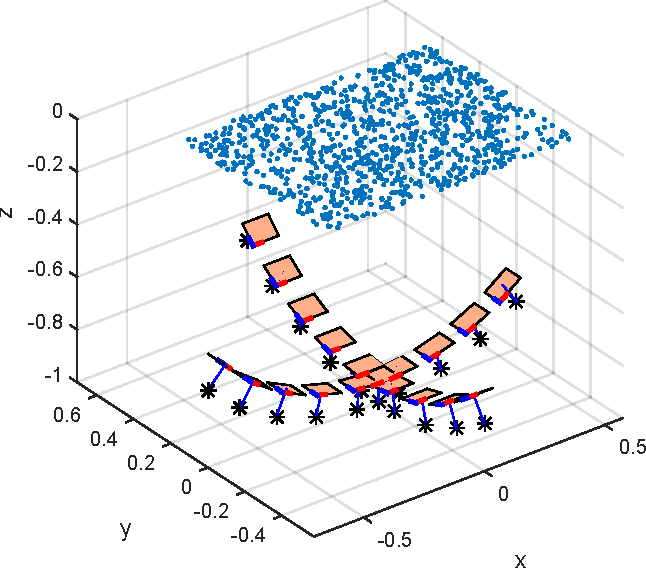
\includegraphics[width=\linewidth]{images/synthCameraPosesRotation.pdf}
	\caption{Scene Fixed-A}
\end{subfigure}
\begin{subfigure}[b]{0.32\linewidth}
	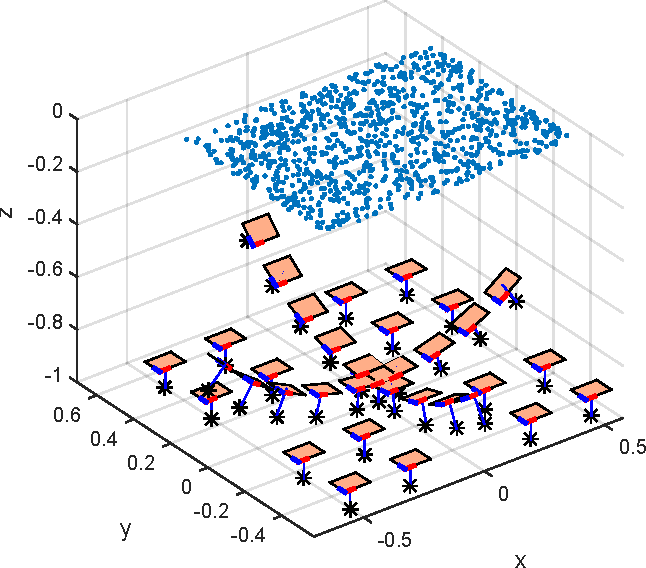
\includegraphics[width=\linewidth]{images/synthCameraPosesTranslation.pdf}
	\caption{Scene Fixed-B}
\end{subfigure}
\begin{subfigure}[b]{0.32\linewidth}
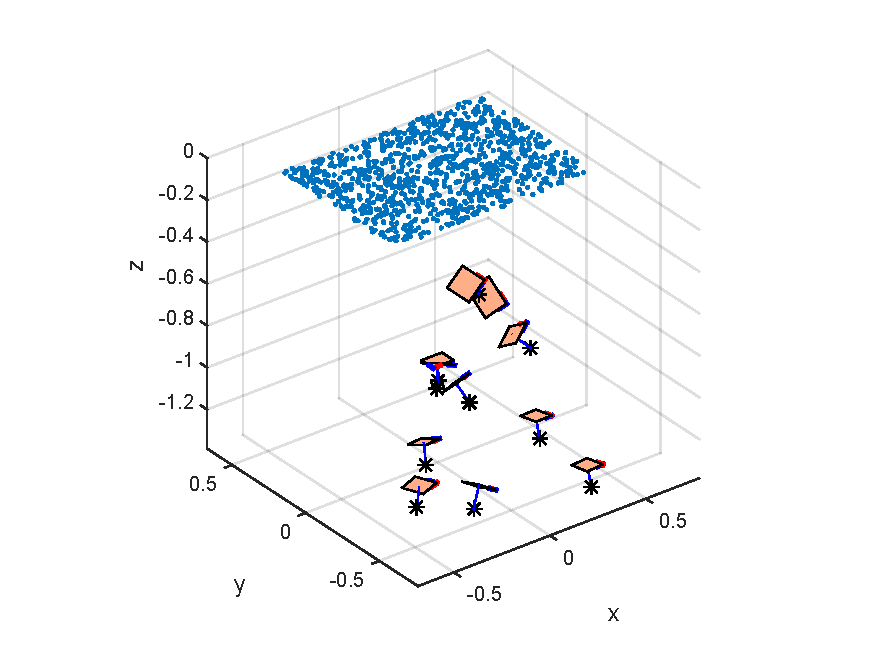
\includegraphics[width=\linewidth]{images/synthCameraPosesRandom.pdf}
	\caption{Scene Random}
\end{subfigure}
\caption{Synthetically generated scenes used for testing. For all scenes $f_x=f_y=600$, $u_0=320$, $v_0=240$, $d_0=0.1$, and $d_1=-0.01$.}
\label{fig:synth_poses}
\end{figure}

Figure \ref{fig:results_normal_angle} shows the robustness of the algorithm to violations of the assumption used to derive the closed-form solution. The reference camera was randomly sampled to have an increasing angle with the scene's plane. We observe that the closed-form focal length estimation was able to produce a good enough initial guess for the system to find the correct calibration with angles of up to $35^\circ$.  Scene \texttt{Fixed-B} was used with noise of $\sigma=1\text{px}$.

\begin{figure}
\centering
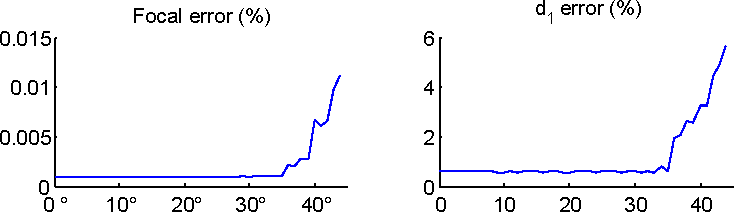
\includegraphics[width=0.7\linewidth]{images/resultsNormalAngle.pdf}
\caption{Robustness of the calibration system to non-perpendicular reference cameras. The calibration is robust to angles of up to $35^\circ$.}
\label{fig:results_normal_angle}
\end{figure}

Figure \ref{fig:results_no_norm} presents a comparison of our normalized constraints with the formulation from \cite{bocquillon2006}. Scene \texttt{Fixed-B} with noise of variable $\sigma$ was used. To show a direct comparison the metric reconstruction stage was disabled, Fig.~\ref{fig:results_no_norm} shows the results after the non-linear minimization of Eq.~\eqref{eq:calib_ba}. The angle between the reference camera and the plane was set to $15^\circ$. The results show that the normalized equations are more accurate and more robust to noise. These results correspond to those obtained by Gurdjos and Sturm \cite{gurdjos2003} with roughly $5\%$ error in the focal length. However, they only tested with small amounts of noise.

\begin{figure}
\centering
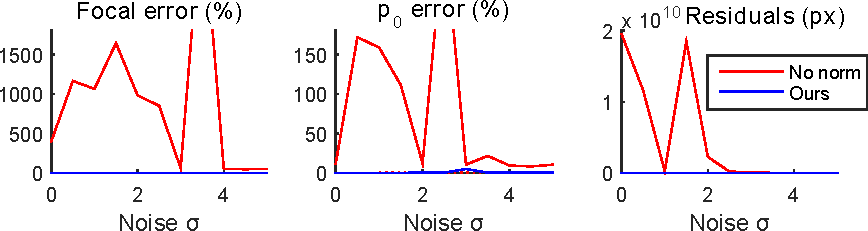
\includegraphics[width=\linewidth]{images/resultsNoNorm2.pdf}
\caption{Comparison of our normalized constraints (blue, coincides with horizontal axis) and those of Bocquillon \cite{bocquillon2006} (red) using $||\Hm||_F=1$. The calibration fails without the normalized constraints, resulting in errors several of magnitude larger. The results shown are after the metric BA, before the BA the results were even worse for \cite{bocquillon2006}. Note that this is the same experiment as in Fig.~\ref{fig:results_noise} but with a different scale.}
\label{fig:results_no_norm}
\end{figure}

Figure \ref{fig:results_noise} evaluates the accuracy of the calibration in the presence of noise. We generate a synthetic scene with noise of increasing $\sigma$. We calibrate using our system (blue solid line for \texttt{Fixed-B} and dotted line for \texttt{Fixed-A}). As a comparison, we also show two cases for scene \texttt{Fixed-B} where the final metic BA is initialized with the ground truth. In the first (green) the points are allowed to vary along the plane, in the second (black) the points are kept fixed at the ground truth to simulate an ideal known-target calibration. 

Figure \ref{fig:results_noise} shows the clear difference in accuracy between scenes \texttt{Fixed-A} and \texttt{Fixed-B}. The translated images help constrain the distortion coefficients and result in a more accurate calibration. We observe that the green line is very close to our results, which means that our calibration is very close the theoretical optimum using planar self-calibration constraints. 
%Importantly, the calibration was improved considerably from that of a purely homography-based self-calibration from Fig.~\ref{fig:results_no_norm}. For noise of $\sigma=1$ we obtain a $500\%$ reduction in the focal length error (from $5\%$ to less than $0.1\%$). This demonstrates the need to have a complete calibration system. 

\begin{figure}
\centering
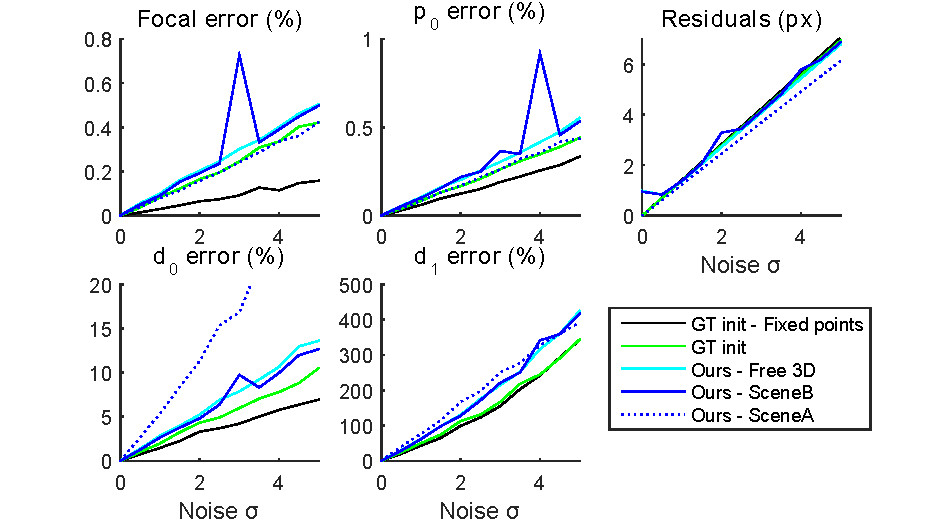
\includegraphics[width=\linewidth]{images/resultsPointNoise2.pdf}
\caption{Comparison of our calibration accuracy with different scenes and increasing noise (blue and red). Results for a final BA initialized from ground truth using fixed (black) and variable (green) scene structure also shown. Our result is only marginally off from the theoretical optimum for self-calibration. Note that this is the same experiment as in Fig.~\ref{fig:results_no_norm} but with a different scale.}
\label{fig:results_noise}
\end{figure}

Self-calibration is more susceptible to noise than a known-target calibration. This is to be expected because it has more degrees of freedom. However, we can correct this by using more images. Fig.~\ref{fig:results_frames} shows the behaviour of the algorithm with a varying number of images used for calibration. We see that the accuracy of the self-calibration converges to that of the known-target calibration when more images are used. For modern cameras it is trivial to capture more images for calibration. In fact, we routinely use a video of the camera moving around looking at a book cover for calibration.

\begin{figure}
\centering
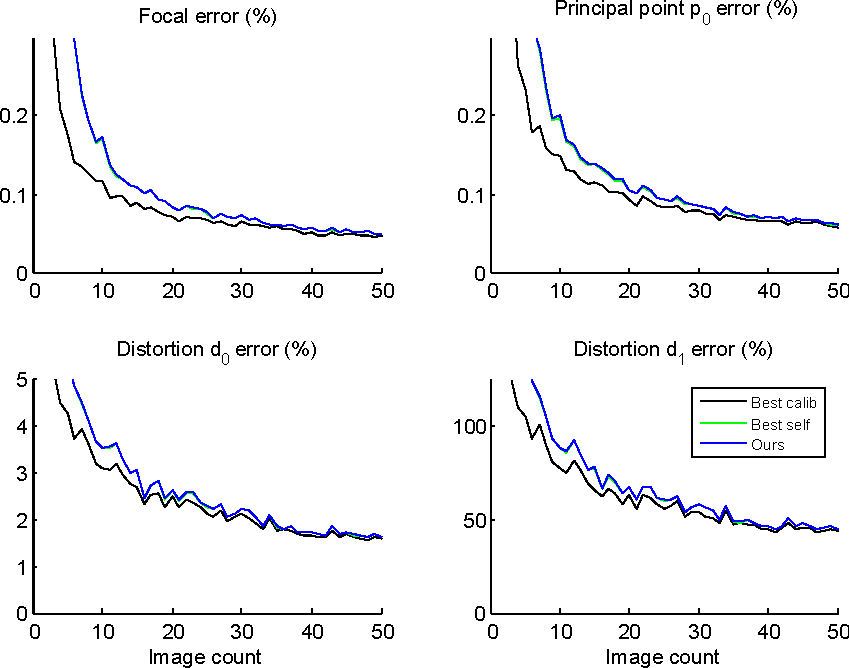
\includegraphics[width=\linewidth]{images/resultsFrameCount.pdf}
\caption{Calibration accuracy with increasing number of images (scene \texttt{Random}, $\sigma=1$). The self-calibration converges with the known-target calibration.}
\label{fig:results_frames}
\end{figure}

%Finally, we show the results of calibrating real cameras using the popular Bouguet toolbox \cite{bouguetMCT} and our method. Bouguet's calibration uses planar checkerboards of known structure to perform calibration. We can therefore use the same input data for our method by ignoring the scene structure and using only the detected image points. Additionally, for the cameras with video capability we perform calibration using a book cover with unknown texture structure. The results are shown in Table \ref{fig:results_real_numbers}. We observe that our method provides an equivalent calibration to that of \cite{bouguetMCT}. We note that although our method is able to calibrate a smartphone's camera, their intrinsics are variable due to autofocus and small variations are to be expected.

%\begin{table*}
%\caption{Comparison of obtained calibrations with real cameras. First column shows the results of calibrating with a checkerboard using Bouguet's toolbox \cite{bouguetMCT}. Second column uses the same detected checkerboard corners to calibrate using our algorithm (without knowledge of 3D structure). Third column uses the video of a book cover to calibrate using our algorithm.}
%\label{fig:results_real_numbers}
%\centering
%\begin{tabular}{|c|c|c|c|c|}
%\hline
%Camera description & & Bouguet toolbox \cite{bouguetMCT} & \multicolumn{2}{|c|}{Our method} \\
% & & & using checkerboard & using book cover \\
% \hline
% Logitech Webcam & $f_x$ & 618.90 & 620.98 & 621.65 \\
%VU-0028 & $f_x$ & 619.28 & 619.67 & 619.63 \\
% & $u_0$ & 316.46 & 318.91 &  307.72 \\
%High-quality VGA & $v_0$ & 238.46 & 231.26 &  229.01 \\
% & $d_0$ & 0.120 & 0.132  &  0.101 \\
%  & $d_1$ & -0.211 & -0.235 &  -0.218 \\
%  \hline
%
%Creative Webcam & $f_x$ & 756.29 & 762.48 & n/a \\
%PD1000 & $f_y$ & 756.75 & 767.78 & n/a \\
%& $u_0$ & 324.31 & 372.52 & n/a \\
%Significant distortion& $v_0$ & 252.10 & 255.69 & n/a \\
%No video available& $d_0$ & -0.390 & -0.665 & n/a \\
%& $d_1$ & 0.197 & 0.524 & n/a \\
%\hline
%
%Smartphone camera & $f_x$ & 1759.96 & 1750.62 & 1765.11 \\
%Google Nexus & $f_y$ & 1758.22 & 1747.53 & 1763.17 \\
%& $u_0$ & 963.80 & 976.07 & 956.92 \\
%High-quality HD& $v_0$ & 541.05 & 534.95 & 550.51 \\
%Refocus during video & $d_0$ & 0.388 & 0.139 & 0.099 \\
%& $d_1$ & -0.674 & -0.601 & -0.423 \\
%\hline
%\end{tabular}
%\end{table*}

\subsection{Real cameras}
We show the results of calibrating real cameras using the popular Bouguet toolbox \cite{bouguetMCT} and our method. Bouguet's calibration uses planar checkerboards of known structure to perform calibration. We use 30 images for calibration and 15 for validation. We use the same hand-picked corner matches for our method without using the known structure to perform a direct comparison. This is shown in Table \ref{fig:results_real_numbers} as \emph{user match}. Additionally, we perform calibration using a video of a flat Lego box with unknown texture structure. ORB features \cite{rublee2011} were automatically matched between frames to provide the necessary correspondences. The results of this video calibration are called \emph{automatic match}. The reprojection error of the calibration images is shown as $e_\text{train}$. The pose of the validation images is optimized and their reprojection error is listed as $e_\text{val}$. 

Our method provides an equivalent calibration to that of \cite{bouguetMCT}. Using the same matches the calibrations are practically identical and the reprojection errors are comparable. Our training reprojection error is marginally lower due to the extra degrees of freedom and the validation error is marginally higher. The obtained accuracy is in line with the synthetic results, showing a 0.15\% focal length error. Moreover, although it is a good reference, the calibration from \cite{bouguetMCT} is not a true ground truth and is also noisy.

For the video sequence, the distortion parameters are considerably underestimated which results in a higher reprojection error. This is due to inaccurate matching and outliers, as indicated by the very high calibration reprojection error. Yet, the reprojection error is still below 1px and the obtained accuracy is better than that reported by \cite{gurdjos2003} which demonstrates the robustness of the calibration approach. The feature matching stage can be improved but it is out of the scope of this paper.

\begin{table}
\caption{Comparison of obtained calibrations using real cameras. Bouguet's values are given as a reference and our calibration is expressed as a relative deviation percentage from it. We achieve practically the same calibration and reprojection errors below 1px on validation.}
\label{fig:results_real_numbers}
\centering
\begin{tabular}{|c|c|c|c|c|}
\hline
& Bouguet \cite{bouguetMCT} & \multicolumn{2}{|c|}{Our method (\%)} \\
& & user match & automatic match  \\
 \hline
$f_x$ & 1384.77 & -0.05 & 0.69 \\
$f_x$ & 1384.92 & -0.15 & 0.93 \\
$u_0$ & 953.78 & -0.27 &  2.00 \\
$v_0$ & 528.42 & -0.41 &  -0.37 \\
$d_0$ & 0.094 & 4.70  &  -37.63 \\
$d_1$ & -0.158 & 2.10 &  -14.45 \\
  \hline
  $e_{\text{train}}$ & 0.25px & 0.23px & 1.94px\\ 
$e_{\text{val}}$ & 0.26px & 0.28px & 0.84px \\ 
  \hline
\end{tabular}
\end{table}

Finally, to showcase the flexibility and applicability of our method we present a simple augmented reality application. A virtual cube is overlaid on top of the scene plane and rigidly attached to it. This is best viewed as a video sequence in the supplemental material
%, but Fig.~\ref{fig:arcube} shows a sample frame
. Plane-based augmented reality is a popular application of computer vision due to its robustness and accuracy. In our case, no knowledge about the plane is needed. The camera can be self-calibrated on the fly and the plane can be augmented with any virtual scene.

%\begin{figure}
%\centering
%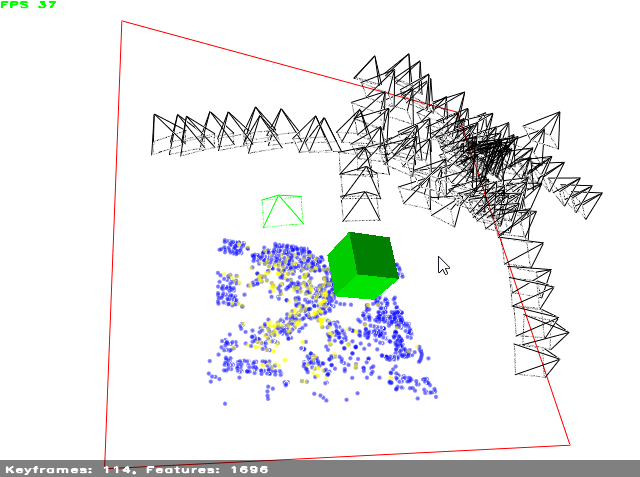
\includegraphics[height=2.3cm]{images/map3d.png}
%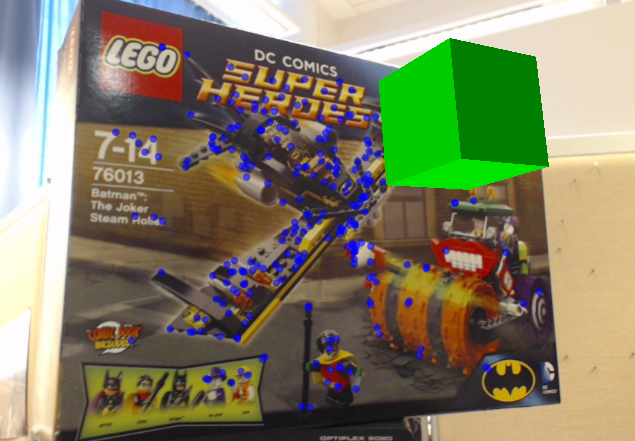
\includegraphics[height=2.3cm]{images/arcube.png}
%\caption{Result of the 3D reconstruction. Left: map of features and cameras. Right: augmented reality on a plane.}
%\label{fig:arcube}
%\end{figure}  

\section{Conclusions}

We have presented a planar self-calibration system that rivals the state-of-the-art calibration algorithms in accuracy and is considerably more practical to use. Our novel derivation of the planar self-calibration constraint shows that the previous formulations are biased. We proposed a set of normalized self-calibration constraints that eliminates this bias and is more robust to noise due to proper normalization. We demonstrated that the assumption used to obtain the closed-form solution to estimate the focal length is not very strict and for most practical purposes poses no limitations on the system. The system proved to be very robust to violations of this assumption, obtaining correct calibrations with angles of up to $35^\circ$ between the reference camera and the scene plane. Our calibration system improves the accuracy of calibration over a purely homography-based self-calibration by over an order of magnitude. 

We showed that our system has such a high accuracy that with enough input images it reaches the same accuracy as a known-target calibration, thus eliminating the practical need of printing checkerboards for camera calibration. As a possible application, our system enables plane-based augmented reality without the need for any prior knowledge about the plane or camera. Finally, we release the code of our calibration system so that the computer vision community can easily adopt this calibration method.

\clearpage

{\small
\bibliographystyle{ieee}
\bibliography{planecalib_paper}
}

\end{document}
